\documentclass[]{article}
\usepackage{graphicx}
\usepackage{float}
\usepackage{indentfirst}
\usepackage{setspace}
\usepackage[hidelinks]{hyperref}

\begin{document}

\begin{titlepage}

\begin{flushleft}
Matteo NOTTARIS and Nicolas BOINAY \\
\bigskip
Tutor : Maria ZULUAGA
\end{flushleft}

\vspace*{\fill}  
\begin{center}  
     {\huge RSI indicator and Machine Learning}\\[30mm]
     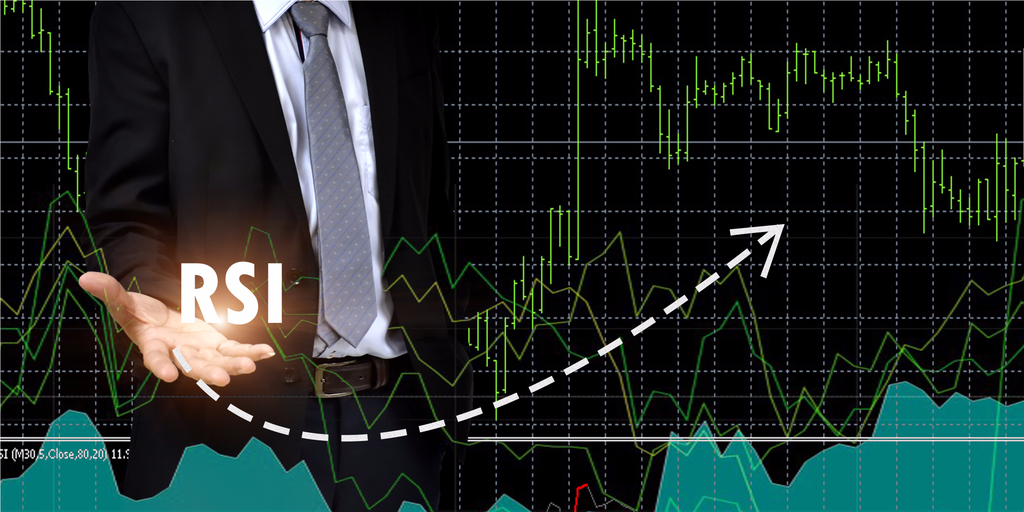
\includegraphics[scale=0.35]{image/rsi_bourse.png}
	 \centering
\end{center}
\vspace*{\fill} 

\end{titlepage}

\doublespacing

\renewcommand*\contentsname{Summary}

\tableofcontents
\clearpage
\singlespacing

\section{Project origin}

\vskip 0.5cm
We wanted to invest ourself in a project which is linked with finance because we both want to orient our professional career in this domain.
In order to do so we contact a FOREX trader working for Crédit Agricole Indosuez Wealth Management, with who one of us worked before during an internship. Our main concern was to find a project's subject which was usable for traders once finished and could have a real application in the trading rooms.

\vskip 0.5cm
We knew that there were already several projects on internet about trying to determine the future evolution of stocks using Machine Learning algorithms. Nevertheless, we wanted for our first ever project in the subject to try something knew, ambitious and above all interesting for traders. Therefore, our contact told us to work on financial indicators which are helping traders to interpret trends on the market.

\vskip 0.5cm 
At the beginning the idea was to right algorithms capable of determining for a given representation of the market the most relevant indicator. Therefore, traders would just need to see which indicator is returned by algorithms and use it in order to interpret a situation. However, we soon understood that it was maybe a bit too complexe for beginners and to develop it in the time we have before the submitting of the project.
Therefore, we slightly change the project to have it as it is today.

\section{Project description}

\vskip 0.5cm
As explained above the project definition slightly change from our original thoughts. We focus on one common and used by traders which is called RSI for Relative Strength Index. RSI is an indicator which gives an indication on the trend of an asset, using two different parameters, which we will call the upper and the lower one. If the RSI signal is over the upper parameter it means that the asset we are interested in (EURUSD in our case) is overbought and therefore there will probably have a reversal in the asset trend. Hence the RSI tells us to sell the asset will the price is high and rebuy it after the reversal, this would allow us to make a profit. The lower parameter is working exactly the same, because when the RSI signal is under it the asset is over sold and the asset trend might go up strongly. As a result the RSI tells us to buy while it is low and sold after the reversal.

\vskip 0.5cm
However, the main problem with this indicator is that it is always used with two parameters like RSI(80,20) or RSI(70,30). We thought that depending on the market situation those two parameters could adapted in order for the RSI to be more precised. 

\vskip 0.5cm
There were three main steps in order to lead this project to its end.\\
The first was to determine what could be a representative picture of a market and then extract all the data sets corresponding.\\
The second one was to find which couple of parameters suits the best for a given situation.\\
With this last step we were able to develop a new data set which we used in our last step of the project which is the training of a Neural Network and find which regression function suits the best our problem.  

\section{Extraction of the data sets}

\vskip 0.5cm
For the good of our project we needed to extract a lot of different data sets (Annexe 1) in order to perfectly determine what represents a market situation. In order to do so we contacted our trader collegue who was far more capable than us to do this list of important representant of the market.\\
We used two different websites to extract the data sets.\\
The first one was \href{https://www.alphavantage.co/}{AlphaVantage} in order to extract the RSI signal for our asset the dual currency EUR/USD.
The second website we used, in order to download the data from all the other stocks, was \href{https://fr.finance.yahoo.com/}{Yahoo Finances}. 

\vskip 0.5cm
The hard part in it wasn't to download the data sets from the websites and load them in excel files, but it was to succeed on making sure that all of them were over the same dates set. Indeed, we needed for one date to be sure that we had the value of each indicators for this given date. We succeeded in doing so, using the manipulation of Python's dictionnaries and arrays.At the end of this step we had more than 2900 common and different dates for all the data set. We could now use this data set as we wanted.

\section{Creation of a new data set}

\vskip 0.5cm
The second step of the project was to generate, using the data sets we downloaded and shaped in the first step, a new data set which would contain for different couple of parameters the most corresponding market situation.

\vskip 0.5cm
In order to do so we had to determine how to estimate the best situation according to a couple of parameters. We decided, with the trader, that the best way was to calcul a performance using the RSI signal and the two chosen parameters. In fact, we are listening to the instructions of the \(RSI(p_1,p_2)\) and we consider that when he tells us to sell we do so end we calcul a performance, in other words we calcul our benefits in percentage, compared to the situation where we would have not listen to it.\\
At the end we look for this given couple of parameters which of the 2900 dates has the highest performance. We did that for every parameter from RSI(90,10) to RSI(51,49) incremented by 0.5 each time. For these 80 different couples we attribute 10 different dates which correspond to the 10 best performances. 

\vskip 0.5cm
This new data set will be used in order to train our Neural Network in the next step of the project. 

\begin{figure}[hbt!]
	\center{}
	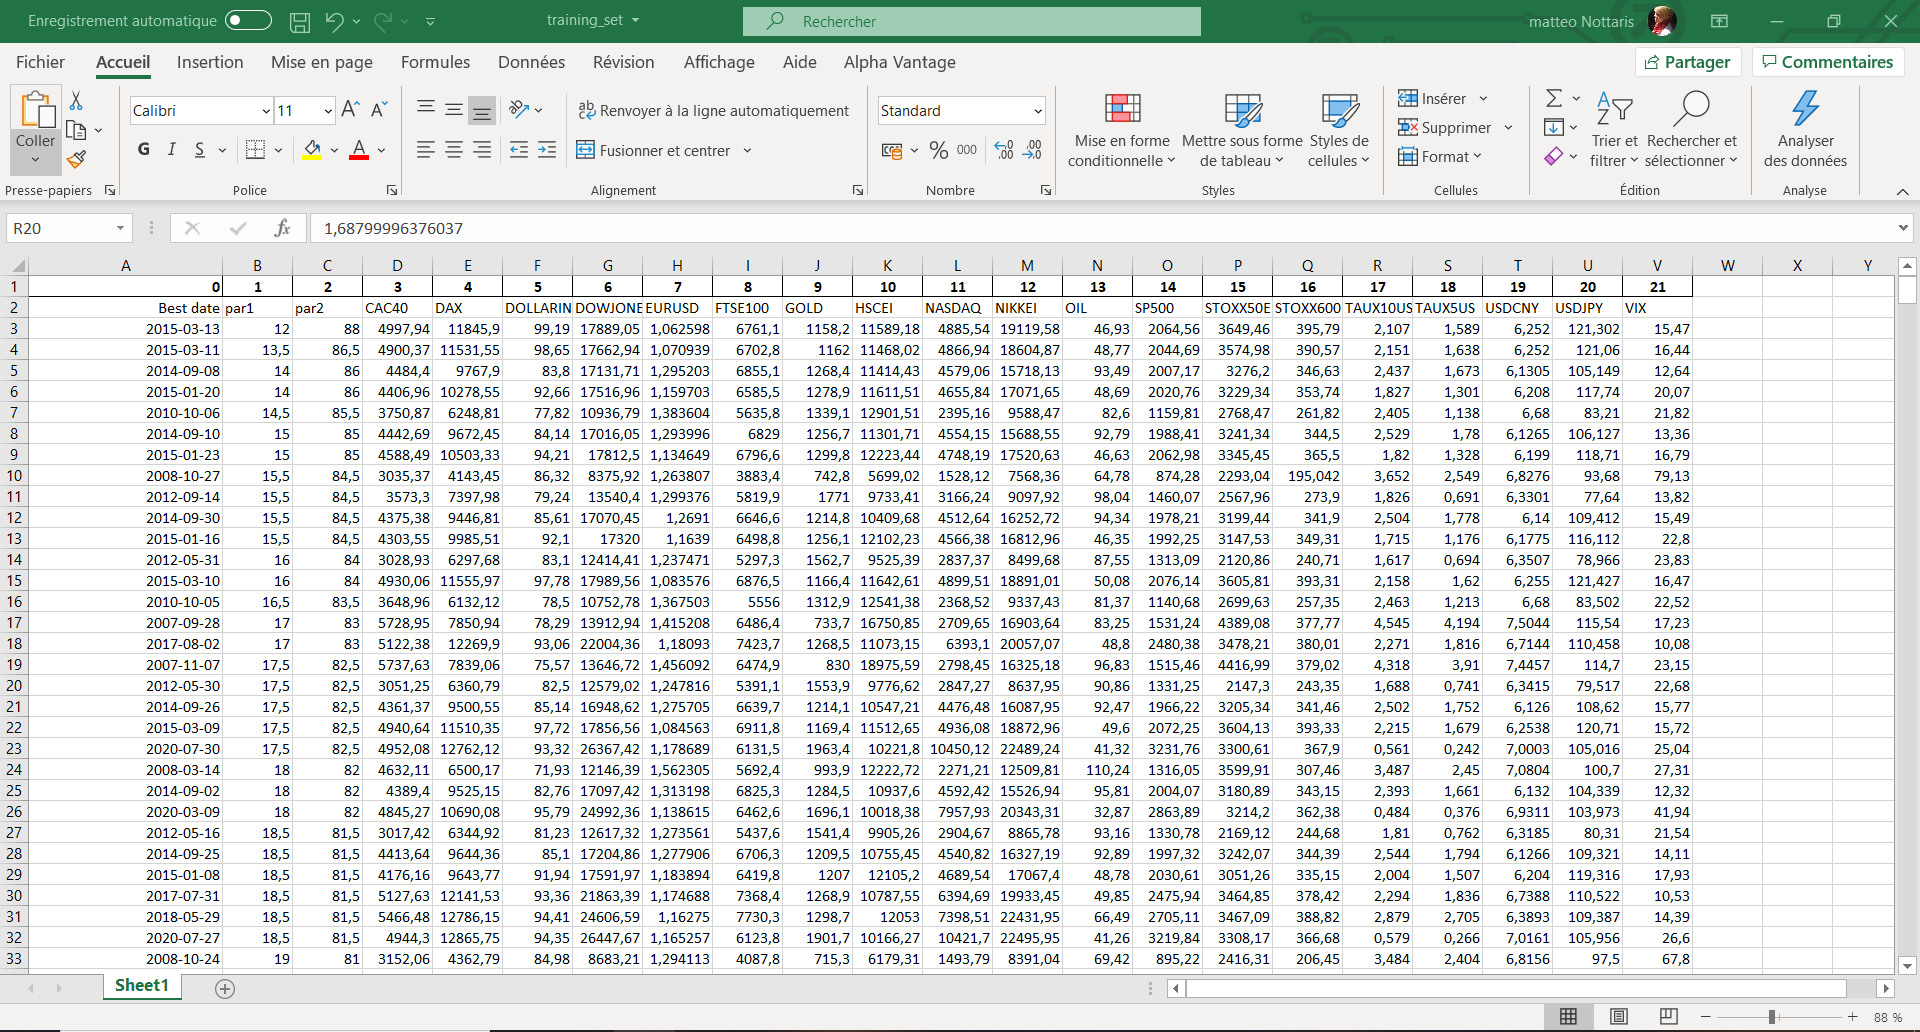
\includegraphics[scale=0.15]{image/training_set.png}
	\caption{New, neural network's training data set}
\end{figure}


\section{Use of a Neural Network}
\vskip 0.5cm
In this last step of the project we are trying to train a neural network. This neural network takes as inputs a vector of shape (19,1), corresponding to the market indicators to define a situation (see Annexe 1). As output the neurak network sends back a vector of shape (2,1) corresponding to the two optimal parameters which should be used considering the situation in input.

\vskip 0.5cm
In order to do so, we took an already implemented neural network that we used during on of our previous labs in class, and tried to adapt it to our situation. \\
The first main difference between the neural network problem in the lab session and our project is that the problem we are tackeling is a regression problem while the other one was a classification exercice. We understood that when we found odd results especially between 0 and 1 due to the sigmoid activation function used.

\vskip 0.5cm
Now that we understood the fact that our problem is a regression one we have changed the activation function on the last layer of our network by a regression function. The next steps in our project is too try many different regression functions and to compare the results between all of them, regarding the error loss. 

\section{Sharing of the work}

\vskip 0.5cm
For the beginning of the project we spread the work pretty evenly.
Nicolas did most of the extraction of data from the two websites (AlphaVantage and Yahoo Finance). 
Then Matteo did the shaping of the data and the creation of the new data set.\\
For now, we are both currently working on the neural network part.

\section{Annexe}
\subsection{Annexe 1} 
\begin{figure}[hbt!]
	\center{}
	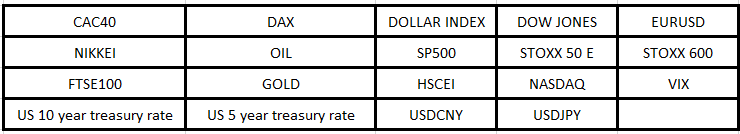
\includegraphics[scale=0.3]{image/marketSituation.png}
	\caption{All market indicators used in our case}
\end{figure}

\end{document}
